\documentclass[NewProceedings,letterpaper]{ascelike-new}
\WarningFilter{caption}{Unknown document class}
\usepackage[utf8]{inputenc}
\usepackage[T1]{fontenc}
\usepackage{graphicx}
\usepackage[style=base,figurename=Fig.,labelfont=bf,labelsep=period]{caption}
\usepackage{amsmath}
\usepackage{newtxtext,newtxmath}
\usepackage{booktabs}
\usepackage{microtype}
\usepackage{needspace}
\usepackage{placeins}
\usepackage[hidelinks]{hyperref}
\captionsetup[figure]{skip=6pt}
\setlength{\belowcaptionskip}{4pt}
\pdfminorversion=7
\graphicspath{{figures/}}
% Generated from reviewer reanalysis v3; do not edit by hand.
\newcommand{\Candidates}{400}
\newcommand{\NumericReferences}{351}
\newcommand{\PositiveReferences}{185}
\newcommand{\ZeroReferences}{154}
\newcommand{\CensoredReferences}{12}
\newcommand{\GeometryExcluded}{44}
\newcommand{\TechnicalExcluded}{5}
\newcommand{\Cells}{140}
\newcommand{\FitCells}{87}
\newcommand{\EvalCells}{64}
\newcommand{\EvalN}{164}
\newcommand{\UtilN}{139}
\newcommand{\AbstainN}{236}
\newcommand{\DomainExcluded}{187}
\newcommand{\ServiceZeros}{28}
\newcommand{\MarginZeros}{38}
\newcommand{\BootstrapN}{5000}
\newcommand{\SeedN}{30}
\newcommand{\PassN}{29}
\newcommand{\HKOriginalN}{13}
\newcommand{\HKRepairedN}{5}
\newcommand{\HKTotalN}{18}
\newcommand{\HKCandidates}{32}
\newcommand{\AffectedReferences}{3}
\newcommand{\CommonPositive}{98}
\newcommand{\MZeroMOnePositive}{38}
\newcommand{\BothZero}{28}
\newcommand{\FlowUntested}{0}
\newcommand{\FlowIncomplete}{0}
\newcommand{\IndependentSeedStart}{10000}
\newcommand{\IndependentSeedEnd}{10029}
\newcommand{\MZeroPositive}{98}
\newcommand{\MZeroZero}{66}
\newcommand{\MZeroExceed}{0}
\newcommand{\MZeroPass}{98}
\newcommand{\MZeroFail}{0}
\newcommand{\MZeroUntested}{0}
\newcommand{\MZeroIncomplete}{0}
\newcommand{\MZeroMAE}{4.54}
\newcommand{\MZeroUtil}{16.7}
\newcommand{\MZeroFailRate}{0.0}
\newcommand{\MZeroUtilLow}{14.3}
\newcommand{\MZeroUtilHigh}{22.5}
\newcommand{\MZeroMeanPositiveQuota}{4.81}
\newcommand{\MZeroMedianPositiveQuota}{5.0}
\newcommand{\MZeroMargin}{3.376}
\newcommand{\MOnePositive}{136}
\newcommand{\MOneZero}{28}
\newcommand{\MOneExceed}{16}
\newcommand{\MOnePass}{118}
\newcommand{\MOneFail}{18}
\newcommand{\MOneUntested}{0}
\newcommand{\MOneIncomplete}{0}
\newcommand{\MOneMAE}{2.43}
\newcommand{\MOneUtil}{75.0}
\newcommand{\MOneFailRate}{13.2}
\newcommand{\MOneUtilLow}{66.7}
\newcommand{\MOneUtilHigh}{80.0}
\newcommand{\MOneMeanPositiveQuota}{6.32}
\newcommand{\MOneMedianPositiveQuota}{5.0}
\newcommand{\MOneMargin}{0.000}
\newcommand{\MTwoPositive}{59}
\newcommand{\MTwoZero}{105}
\newcommand{\MTwoExceed}{0}
\newcommand{\MTwoPass}{59}
\newcommand{\MTwoFail}{0}
\newcommand{\MTwoUntested}{0}
\newcommand{\MTwoIncomplete}{0}
\newcommand{\MTwoMAE}{6.98}
\newcommand{\MTwoUtil}{0.0}
\newcommand{\MTwoFailRate}{0.0}
\newcommand{\MTwoUtilLow}{0.0}
\newcommand{\MTwoUtilHigh}{5.3}
\newcommand{\MTwoMeanPositiveQuota}{1.19}
\newcommand{\MTwoMedianPositiveQuota}{1.0}
\newcommand{\MTwoMargin}{5.106}
\newcommand{\MThreePositive}{98}
\newcommand{\MThreeZero}{66}
\newcommand{\MThreeExceed}{2}
\newcommand{\MThreePass}{96}
\newcommand{\MThreeFail}{2}
\newcommand{\MThreeUntested}{0}
\newcommand{\MThreeIncomplete}{0}
\newcommand{\MThreeMAE}{4.55}
\newcommand{\MThreeUtil}{18.2}
\newcommand{\MThreeFailRate}{2.0}
\newcommand{\MThreeUtilLow}{15.4}
\newcommand{\MThreeUtilHigh}{20.0}
\newcommand{\MThreeMeanPositiveQuota}{4.83}
\newcommand{\MThreeMedianPositiveQuota}{5.0}
\newcommand{\MThreeMargin}{3.429}
\newcommand{\MainC}{23.842}
\newcommand{\MainP}{-0.930}
\newcommand{\WidthExponent}{1.930}
\newcommand{\MAEDifference}{-0.012}
\newcommand{\MAEDifferenceLow}{-0.043}
\newcommand{\MAEDifferenceHigh}{0.019}
\newcommand{\UtilDifference}{58.3}
\newcommand{\UtilDifferenceLow}{47.7}
\newcommand{\UtilDifferenceHigh}{63.3}
\newcommand{\AccessDifference}{38}
\newcommand{\FailDifference}{18}
\newcommand{\Coverage}{41.0}
\newcommand{\HKCoverage}{56.2}
\newcommand{\CommonMZeroPass}{98}
\newcommand{\CommonMZeroFail}{0}
\newcommand{\CommonMZeroUntested}{0}
\newcommand{\CommonMOnePass}{86}
\newcommand{\CommonMOneFail}{12}
\newcommand{\CommonMOneUntested}{0}
\newcommand{\HKOrigMZeroPass}{7}
\newcommand{\HKOrigMZeroFail}{0}
\newcommand{\HKOrigMZeroUntested}{0}
\newcommand{\HKOrigMZeroPositive}{7}
\newcommand{\HKOrigMZeroZero}{6}
\newcommand{\HKOrigMZeroExceed}{0}
\newcommand{\HKOrigMZeroUtilN}{10}
\newcommand{\HKOrigMZeroUtil}{16.7}
\newcommand{\HKOrigMOnePass}{10}
\newcommand{\HKOrigMOneFail}{1}
\newcommand{\HKOrigMOneUntested}{0}
\newcommand{\HKOrigMOnePositive}{11}
\newcommand{\HKOrigMOneZero}{2}
\newcommand{\HKOrigMOneExceed}{1}
\newcommand{\HKOrigMOneUtilN}{10}
\newcommand{\HKOrigMOneUtil}{64.6}
\newcommand{\HKOrigMTwoPass}{7}
\newcommand{\HKOrigMTwoFail}{0}
\newcommand{\HKOrigMTwoUntested}{0}
\newcommand{\HKOrigMTwoPositive}{7}
\newcommand{\HKOrigMTwoZero}{6}
\newcommand{\HKOrigMTwoExceed}{0}
\newcommand{\HKOrigMTwoUtilN}{10}
\newcommand{\HKOrigMTwoUtil}{8.3}
\newcommand{\HKOrigMThreePass}{7}
\newcommand{\HKOrigMThreeFail}{0}
\newcommand{\HKOrigMThreeUntested}{0}
\newcommand{\HKOrigMThreePositive}{7}
\newcommand{\HKOrigMThreeZero}{6}
\newcommand{\HKOrigMThreeExceed}{0}
\newcommand{\HKOrigMThreeUtilN}{10}
\newcommand{\HKOrigMThreeUtil}{16.7}
\newcommand{\HKRepairMZeroPass}{4}
\newcommand{\HKRepairMZeroFail}{0}
\newcommand{\HKRepairMZeroUntested}{0}
\newcommand{\HKRepairMZeroPositive}{4}
\newcommand{\HKRepairMZeroZero}{1}
\newcommand{\HKRepairMZeroExceed}{0}
\newcommand{\HKRepairMZeroUtilN}{5}
\newcommand{\HKRepairMZeroUtil}{20.0}
\newcommand{\HKRepairMOnePass}{5}
\newcommand{\HKRepairMOneFail}{0}
\newcommand{\HKRepairMOneUntested}{0}
\newcommand{\HKRepairMOnePositive}{5}
\newcommand{\HKRepairMOneZero}{0}
\newcommand{\HKRepairMOneExceed}{0}
\newcommand{\HKRepairMOneUtilN}{5}
\newcommand{\HKRepairMOneUtil}{50.0}
\newcommand{\HKRepairMTwoPass}{2}
\newcommand{\HKRepairMTwoFail}{0}
\newcommand{\HKRepairMTwoUntested}{0}
\newcommand{\HKRepairMTwoPositive}{2}
\newcommand{\HKRepairMTwoZero}{3}
\newcommand{\HKRepairMTwoExceed}{0}
\newcommand{\HKRepairMTwoUtilN}{5}
\newcommand{\HKRepairMTwoUtil}{0.0}
\newcommand{\HKRepairMThreePass}{4}
\newcommand{\HKRepairMThreeFail}{0}
\newcommand{\HKRepairMThreeUntested}{0}
\newcommand{\HKRepairMThreePositive}{4}
\newcommand{\HKRepairMThreeZero}{1}
\newcommand{\HKRepairMThreeExceed}{0}
\newcommand{\HKRepairMThreeUtilN}{5}
\newcommand{\HKRepairMThreeUtil}{20.0}
\newcommand{\DevBaselineRows}{11850}
\newcommand{\DevBaselineZero}{1370}
\newcommand{\DevBaselinePlanned}{1459920}
\newcommand{\DevBaselineObserved}{1414320}
\newcommand{\DevBaselineNever}{64770}
\newcommand{\DevMixedRows}{65671}
\newcommand{\DevMixedZero}{2116}
\newcommand{\DevMixedPlanned}{7507512}
\newcommand{\DevMixedObserved}{7506852}
\newcommand{\DevMixedNever}{660}
\newcommand{\HKBaselineRows}{540}
\newcommand{\HKBaselineZero}{60}
\newcommand{\HKBaselinePlanned}{63600}
\newcommand{\HKBaselineObserved}{63600}
\newcommand{\HKBaselineNever}{0}
\newcommand{\HKMixedRows}{4770}
\newcommand{\HKMixedZero}{307}
\newcommand{\HKMixedPlanned}{638400}
\newcommand{\HKMixedObserved}{638400}
\newcommand{\HKMixedNever}{0}
\newcommand{\ContinuousMZeroMedianSpeed}{0.982}
\newcommand{\ContinuousMOneMedianSpeed}{0.963}
\newcommand{\ContinuousMZeroWorst}{0.883}
\newcommand{\ContinuousMOneWorst}{0.071}
\newcommand{\TimeStep}{0.1}
\newcommand{\Warmup}{100}
\newcommand{\Measurement}{240}
\newcommand{\Tail}{100}
\newcommand{\PedSpeed}{1.25}
\newcommand{\PedSD}{0.15}
\newcommand{\PedMin}{0.8}
\newcommand{\PedMax}{1.8}
\newcommand{\PedRadius}{0.25}
\newcommand{\RobotLength}{0.96}
\newcommand{\RobotWidth}{0.7}
\newcommand{\RobotRadius}{0.48}
\newcommand{\RobotSpeed}{1.39}
\newcommand{\CorridorLength}{50}
\newcommand{\ZoneLength}{20}
\newcommand{\WindowEnd}{340}
\newcommand{\Timeout}{300}
\newcommand{\QMax}{20}
\newcommand{\WidthMin}{1.6}
\newcommand{\WidthMax}{3}
\newcommand{\DemandMax}{60}
\newcommand{\SpeedFloor}{0.8}
\newcommand{\SpeedRetention}{0.90}
\newcommand{\DensityLimit}{1.20}
\newcommand{\FlowLow}{0.90}
\newcommand{\FlowHigh}{1.20}
\newcommand{\Quantile}{0.80}
\newcommand{\SpecificMax}{33.33}
\newcommand{\SinuosityMax}{1.05}
\newcommand{\TurnAngle}{20}
\newcommand{\TurnRatio}{0.6}
\newcommand{\NarrowWidth}{1.75}
\newcommand{\NarrowDefaultPass}{30}
\newcommand{\NarrowSmallPass}{30}
\newcommand{\NarrowLargePass}{0}
\newcommand{\NarrowDirectionPass}{28}
\newcommand{\WideWidth}{2.4}
\newcommand{\WideDefaultPass}{30}
\newcommand{\WideSmallPass}{30}
\newcommand{\WideLargePass}{30}
\newcommand{\WideDirectionPass}{29}
\newcommand{\SensitivityFlow}{4}
\newcommand{\SmallRadius}{0.385}
\newcommand{\LargeRadius}{0.575}
\newcommand{\Cities}{7}
\newcommand{\TrainCities}{6}
\newcommand{\MainScenarios}{280}
\newcommand{\AdditionalScenarios}{120}
\newcommand{\EvalCensored}{8}
\newcommand{\HKExcluded}{14}
\newcommand{\RepairClearance}{0.75}
\newcommand{\HKOriginalCoverage}{40.6}
\newcommand{\MeanSeedsPooled}{30}
\newcommand{\EngineVersion}{SUMO 1.27.1}
\newcommand{\ConfidenceLevel}{95}
\newcommand{\FlowGrid}{1, 2, 3, 4, 5, 6, 8, 10, 12, 15, 18, 20}
\newcommand{\WithdrawnPass}{32}
\newcommand{\WithdrawnFail}{6}
\newcommand{\CommonMZeroMean}{4.81}
\newcommand{\CommonMOneMean}{7.55}

\setlength{\textfloatsep}{12pt plus 2pt minus 2pt}
\setlength{\intextsep}{12pt plus 2pt minus 2pt}
\renewcommand{\topfraction}{0.9}
\renewcommand{\bottomfraction}{0.8}
\renewcommand{\textfraction}{0.08}
\renewcommand{\floatpagefraction}{0.90}
\NameTag{}
\begin{document}
\clubpenalty=10000 \widowpenalty=10000
\title{Balancing Pedestrian Service and Robot Access: An Interpretable Admission Framework for Sidewalk Delivery Robots}
\author[1]{An Xu}
\author[1,*]{Yunfei Yin}
\affil[1]{School of Transportation Science and Engineering,
Harbin Institute of Technology, Harbin 150090, China}
\affil[ ]{\texttt{AnX.RTL2324@tum-asia.edu.sg} (An Xu);
\texttt{yunfeiyin@hit.edu.cn} (Yunfei Yin)}
\maketitle
\begingroup
\renewcommand{\thefootnote}{*}
\footnotetext[0]{Corresponding author: Yunfei Yin (yunfeiyin@hit.edu.cn).}
\endgroup
\begin{abstract}
Operating permission for sidewalk delivery robots leaves a local allocation question: how much robot entry flow can a sidewalk accommodate under a stated pedestrian-service objective? We develop an admission framework that checks applicability and pedestrian baseline service before estimating a candidate entry rate from width and demand. City-held-out evaluation compares conservative allocation with alternative estimators. All positive recommendations were tested directly at their specified flows. Across \EvalN{} scenarios, the margin-based method offered \MZeroPositive{} positive recommendations, with \MZeroPass{} passes and \MZeroFail{} failures. Removing the margin increased access to \MOnePositive{} positive recommendations, with \MOnePass{} passes and \MOneFail{} failures. Median reference utilization increased from \MZeroUtil{}\% to \MOneUtil{}\%. Of the \MZeroMOnePositive{} additional opportunities, \WithdrawnPass{} passed and \WithdrawnFail{} failed, showing the access cost of conservative allocation. An unconstrained width--demand estimator produced similar aggregate outcomes to the margin-based method. Transfer to \HKOriginalN{} original and \HKRepairedN{} entrance-repaired Hong Kong configurations extended the analysis to irregular polygons. Geometry, robot size, and flow composition affected applicability. The framework supports service-aware evaluation of robot access under specified operating conditions.
\end{abstract}

\Needspace{6\baselineskip}
\section{Introduction}
U.S. states including Virginia and Washington permit sidewalk delivery devices under specified operating conditions \cite{VirginiaPDD,WashingtonPDD}. Singapore has enabled supervised public-path trials through regulatory exemptions \cite{LTAExemptions,IMDAPunggol}. These arrangements address operation and pedestrian protection; the District of Columbia also limits fleet size in initial permits \cite{DDOTPDD}. Yet operating permission and fleet limits do not determine how many robots per minute should enter a particular sidewalk. That decision depends on local width, pedestrian demand, and the service that walking should retain.

Delivery robots offer potential freight benefits \cite{Jennings2019}, but each movement shares space primarily used by pedestrians. Research has examined robot regulation and deployment \cite{Kovacica2024}, pedestrian interactions \cite{Gehrke2022}, and delivery routing under uncertain travel conditions \cite{TongSimoni2026}. These studies motivate a related traffic-engineering question: how much robot access should be offered on a defined sidewalk under a stated pedestrian-service objective? The decision variable here is a segment entry rate, measured in robots/min.

A regression estimate alone leaves several decisions unresolved. Some geometries lie outside the assessed domain. Some pedestrian-only conditions already fail the service criterion. Other conditions support a positive robot recommendation, but the amount offered depends on how conservatively the available space is allocated. These cases call for different responses: further assessment, zero admission, or a candidate entry rate linked to a service test.

We develop an interpretable framework that connects these responses through applicability checks, a pedestrian-service gate, and a width--demand estimate with a margin. City-held-out comparisons quantify how conservativeness changes robot access and pedestrian-service outcomes. Tests with frozen development parameters examine transfer to Hong Kong sidewalk polygons. The contributions are an explicit admission decision structure, a direct comparison of access and service at recommended flows, and an assessment of the conditions that limit geometric transfer.

\begin{figure}[!htbp]
\centering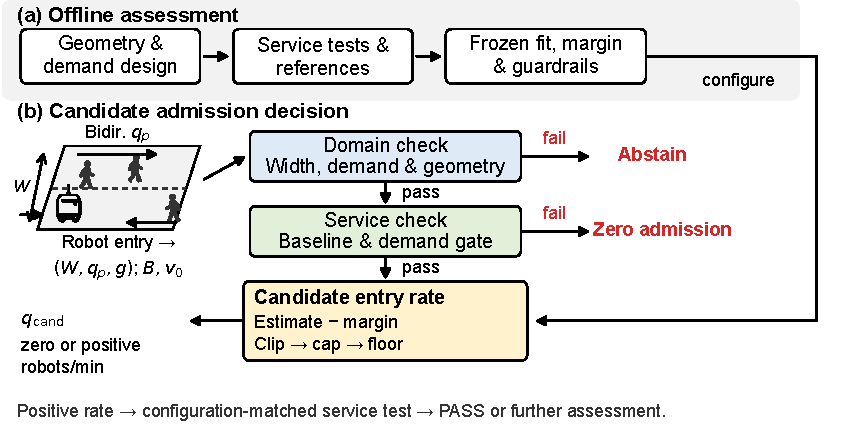
\includegraphics[width=\textwidth]{figures/figure1.pdf}
\caption{Admission decision structure. Applicability determines whether a scenario can be assessed. Pedestrian baseline and demand checks precede candidate-rate calculation. A positive candidate proceeds to a service test at the specified configuration and flow.}
\label{fig:framework}
\end{figure}

\Needspace{6\baselineskip}
\section{From Pedestrian Service to Robot Access}
\Needspace{4\baselineskip}
\subsection{Study Scenarios}
The study contains \Candidates{} geometry--demand scenarios from \Cells{} sidewalk cells in Amsterdam, Melbourne, New Taipei, New York, Seattle, Taipei, and Taoyuan. GIS-derived widths and centreline descriptors define idealized corridors of nominal length \CorridorLength{}~m. The \MainScenarios{} main scenarios use demand priors informed by nearby residential, commercial, tourism, and transit activity. Another \AdditionalScenarios{} scenarios extend the demand range. Demand is specified for the experiments rather than measured as pedestrian arrivals in these cities.

Simulations use \EngineVersion{} with JuPedSim \cite{Lopez2018}. Robots are represented as walking agents with dimensions \RobotLength{} by \RobotWidth{}~m, interaction radius \RobotRadius{}~m, and nominal speed \RobotSpeed{}~m/s. Pedestrians have radius \PedRadius{}~m. Their desired speeds have mean \PedSpeed{}~m/s and standard deviation \PedSD{}~m/s, bounded by \PedMin{} and \PedMax{}~m/s. Pedestrian demand is divided equally between directions, and robots enter in one direction. Regular scheduled arrivals specify demand; random seeds vary stochastic agent properties.

Each run uses a \TimeStep{}~s time step, a \Warmup{}~s warm-up, and a \Measurement{}~s measurement window. A further \Tail{}~s allows trips to finish and is excluded from service measurement. A central \ZoneLength{}~m zone defines the speed and density measurements. In irregular polygons, positions are projected onto the measurement axis. Zone length multiplied by representative width supplies the density denominator.

Physical feasibility is checked before service evaluation. Eroding the walkable polygon by the robot radius leaves no feasible centre region in \GeometryExcluded{} scenarios. A further \TechnicalExcluded{} pedestrian-only runs exceed the \Timeout{}~s wall-clock limit and lack completed measurements. These two groups are excluded rather than assigned zero admission. Completed runs with congestion retain their adverse service outcomes.

\Needspace{4\baselineskip}
\subsection{Pedestrian-Service Criterion}
The service objective combines pedestrian speed retention, density, and a completed-trip flow ratio. For seed $s$, mean speed $\bar v_s$ averages pedestrian observations in the measurement zone and window. Mean density $\bar k_s$ averages the pedestrian count divided by zone area. Robots are excluded from both measures. Baseline speed $v_0$ is the mean of the pedestrian-only seed means for the same scenario and configuration. A mixed-flow seed qualifies when
\begin{equation}
 \bar v_s/v_0\geq\SpeedRetention{},\qquad
 \bar k_s\leq\DensityLimit{},\qquad
 \FlowLow{}\leq T_s\leq\FlowHigh{}.
 \label{eq:service}
\end{equation}
Density is in ped/m$^2$. The thresholds express the study's service objective. Speed retention compares each mixed-flow seed with a common baseline mean.

The flow ratio is $T_s=N_{\rm arr,s}^{\rm comp}/N_{\rm dep,s}^{\rm comp}$. Its numerator counts completed pedestrian records arriving during measurement; its denominator counts completed records departing during measurement. When the denominator is zero, $T_s$ is undefined and the seed fails this component. Scheduled agents, first observations, completed trips, and window stocks are retained as separate demand diagnostics. First observation establishes visibility to the simulator, not an exact insertion time into the walking model.

A flow qualifies when at least \PassN{} of \SeedN{} seeds satisfy Eq.~\ref{eq:service}. Pedestrian-only qualification $B$ applies the density and flow-ratio criteria with the same acceptance count. All primary references use seeds 0--29. Independent seeds \IndependentSeedStart{}--\IndependentSeedEnd{} are used only for replication, with a separate baseline mean.

The simulation reference $q^*$ is the highest qualifying flow in the reference scan. It is zero when no tested flow qualifies and is censored at the \QMax{}~robots/min ceiling. Coarse design flows are \FlowGrid{}~robots/min; higher levels and integer refinements are applied selectively. Scan support can differ among scenarios. Later recommendation tests are evaluated separately from reference construction. The resulting sample contains \PositiveReferences{} positive uncensored references, \ZeroReferences{} zeros, and \CensoredReferences{} ceiling-censored references.

\Needspace{4\baselineskip}
\subsection{Admission Decision}
Figure~\ref{fig:framework} connects service evaluation to robot access. Inputs are clear width $W$, pedestrian demand $q_p$, geometry descriptors $g$, baseline qualification $B$, and baseline speed $v_0$. Applicability is assessed first. Missing inputs, invalid evidence, or a scenario outside the assessed domain produce abstention.

The domain $\mathcal D$ covers widths of \WidthMin{}--\WidthMax{}~m and positive pedestrian demand no greater than \DemandMax{}~ped/min. Specific demand is $x=q_p/W<\SpecificMax{}$~ped/min/m. Straight and mildly curved geometries are included up to sinuosity \SinuosityMax{}. Concentrated turns are excluded when maximum and cumulative angles both reach \TurnAngle{} degrees and their ratio reaches \TurnRatio{}.

For an assessable scenario, the pedestrian-service gate $G$ requires $B=1$, $v_0\geq\SpeedFloor{}$~m/s, and $q_p<C(W)$. Failure of this gate returns zero admission. Otherwise, the method subtracts a margin from the nominal estimate, applies flow ceilings, and rounds down:
\begin{equation}
q_{\rm cand}=
\begin{cases}
\text{abstain},&\text{inputs invalid or }(W,q_p,g)\notin\mathcal D,\\
0,&(W,q_p,g)\in\mathcal D,\ G=0,\\
\lfloor\min\{q_{\max},Q_{\rm low}(W),[q_{\rm nom}-\Delta]_+\}\rfloor,
 &(W,q_p,g)\in\mathcal D,\ G=1.
\end{cases}
\label{eq:quota}
\end{equation}
Here $[z]_+=\max(0,z)$ and $q_{\max}=\QMax{}$~robots/min. Margin subtraction and rounding may also produce zero. This distinguishes a pedestrian-service gate from a conservative allocation decision. A positive output is a candidate entry rate for configuration-matched testing.

The margin-based method M0 uses the width--demand estimate
\begin{equation}
 q_{\rm nom}=cW(q_p/W)^p,\qquad
 \log(q^*/W)=\log c+p\log x+\varepsilon.
 \label{eq:nominal}
\end{equation}
Ordinary least squares fits positive uncensored training references. Zero and ceiling-censored references are omitted from this logarithmic fit but retained in margin calibration. The margin $\Delta$ is the \Quantile{} quantile of $[q_{\rm nom}-q^*]_+$ across training scenarios with defined references. Fitting and margin calibration use the recorded rounded $x$ values. Candidate-rate calculation evaluates $q_p/W$ from the stored inputs.

\begin{table}[!htbp]
\centering\caption{Demand gate and low-demand ceiling, interpolated linearly between width knots.}
\label{tab:guards}\begin{tabular}{lrrrrrrr}
\toprule
$W$ (m) & 1.6 & 1.7 & 1.8 & 2.1 & 2.4 & 2.7 & 3 \\
\midrule
$C(W)$ (ped/min) & 35.0 & 35.0 & 45.0 & 45.0 & 55.0 & 90.0 & 90.0 \\
$Q_{\rm low}(W)$ (robots/min) & 5.0 & 6.0 & 8.0 & 10.0 & 18.0 & 20.0 & 20.0 \\
\bottomrule
\end{tabular}

\end{table}
The demand gate $C(W)$ and low-demand ceiling $Q_{\rm low}(W)$ were established from the synthetic grid and held fixed (Table~\ref{tab:guards}). They supplement the fitted relation by limiting the range of offered access.

\Needspace{6\baselineskip}
\section{Evaluation Design}
\Needspace{4\baselineskip}
\subsection{City-Held-Out Comparison}
Four methods share the same applicability checks, service gate, and ceilings. M1 removes the margin from M0, setting $\Delta=0$. It isolates the effect of conservative allocation within this framework. M2 uses a width-only relation, $\log q_{\rm nom}=a+b\log W$, with its own calibrated margin. M3 uses the unconstrained relation $\log q_{\rm nom}=a+b\log W+d\log q_p$, also with its own margin. M0 imposes $b+d=1$ in this representation. M0 has two fitted coefficients and M3 has three.

Each of the \Cities{} folds fits coefficients and margin on \TrainCities{} cities and predicts the remaining city. All cells from the held-out city are excluded from fitting. The previously selected gates and ceilings remain fixed across folds. Applicability screening leaves \EvalN{} scenarios from \EvalCells{} unique cells, or \Coverage{}\% of the candidate sample. The \AbstainN{} abstentions comprise \GeometryExcluded{} physical exclusions, \TechnicalExcluded{} technical exclusions, and \DomainExcluded{} operational-domain exclusions. Zero recommendations remain in the evaluation population.

\Needspace{4\baselineskip}
\subsection{Direct Recommendation Tests}
The primary outcomes are robot access and pedestrian-service outcomes at the recommended flow. We report positive and zero recommendations on the common scenario set. Positive flows are matched to tests by scenario, entrance configuration, flow, and original seed block. Methods recommending the same flow share its test evidence. A complete \SeedN{}-seed group produces PASS or FAIL according to Eq.~\ref{eq:service}. All positive recommendations have complete configuration-matched tests. Zero admission is not counted as a service pass.

Mean positive candidate flow describes the amount of access offered in robots/min. It is a nominal recommendation, separate from completed robot throughput. To describe pedestrian service continuously, we also summarize seed-level speed retention within tested groups.

Reference exceedance counts recommendations with $q_{\rm cand}>q^*$. Mean absolute error (MAE) compares candidate rates with $q^*$ on all \EvalN{} evaluated scenarios. Reference utilization is
\begin{equation}
 U=\operatorname{median}_{i:\,q_i^*>0}
       \left(q_{{\rm cand},i}/q_i^*\right).
 \label{eq:utilization}
\end{equation}
Its denominator includes \UtilN{} scenarios with positive references, including \EvalCensored{} ceiling-censored references. Zero recommendations remain in the median, and ratios above unity are not clipped. Direct service tests and reference comparisons answer different questions: a recommendation can lie below $q^*$ yet fail at its own tested flow.

Uncertainty intervals use \BootstrapN{} paired cell-cluster resamples with replacement. Predictions, margins, and references remain fixed. The \ConfidenceLevel{}\% percentile intervals describe variation in site composition; they exclude retraining and simulation-seed uncertainty.

\Needspace{4\baselineskip}
\subsection{Geometry Transfer to Hong Kong}
The transfer experiment applies development parameters to irregular sidewalk polygons. Fitting on the full development set gives M0 parameters $c=\MainC{}$, $p=\MainP{}$, and $\Delta=\MZeroMargin{}$~robots/min. These parameters and the other methods' margins are frozen before the reported transfer calculations. Hong Kong data contribute to neither coefficient fitting nor margin selection.

The sample contains \HKCandidates{} candidate polygons. Domain screening retains \HKTotalN{} sites, of which \HKOriginalN{} use original entrance configurations. The remaining \HKRepairedN{} use entrance repairs within the original polygon. Repair moves entrance anchors to the nearest feasible points after erosion by \RepairClearance{}~m and aligns the entrance stubs with the principal axis. Polygon shape, representative width, measurement axis, agent properties, and demand are retained. Each polygon contributes one final configuration. Original and repaired configurations are evaluated separately with matching baselines.

\Needspace{6\baselineskip}
\section{Results}
\Needspace{4\baselineskip}
\subsection{Conservativeness Trades Robot Access for Pedestrian Service}
Removing the margin offered robot access in more scenarios and produced more failed service tests (Fig.~\ref{fig:reference}; Table~\ref{tab:loco}). M0 issued \MZeroPositive{} positive recommendations and \MZeroZero{} zeros. Its positive recommendations included \MZeroPass{} passes and \MZeroFail{} failures. M1 issued \MOnePositive{} positives and \MOneZero{} zeros, with \MOnePass{} passes and \MOneFail{} failures. Positive access increased by \AccessDifference{} scenarios when the margin was removed.

\begin{figure}[!htbp]
\centering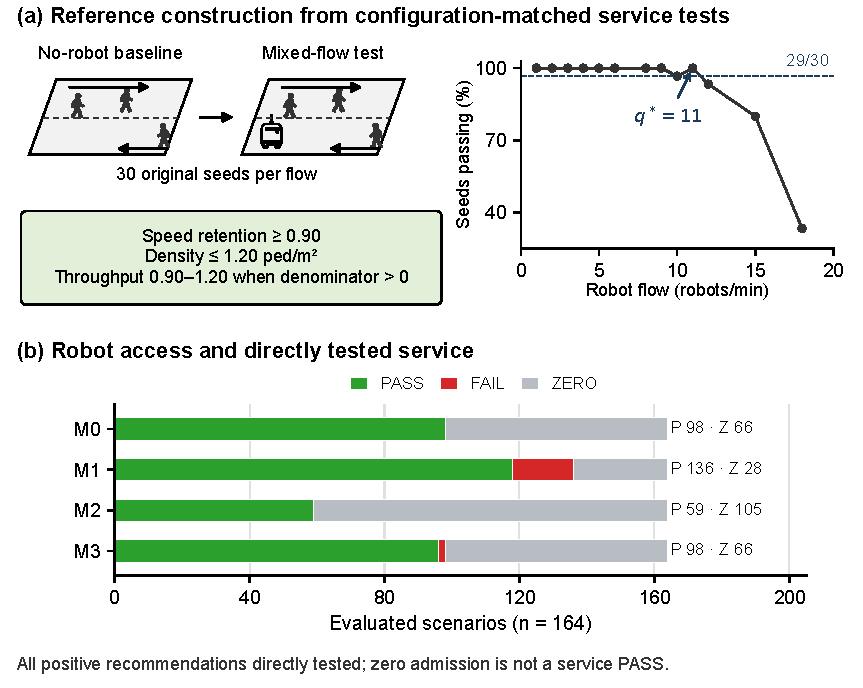
\includegraphics[width=\textwidth]{figures/figure2.pdf}
\caption{Pedestrian service and robot access. (a) Baseline and mixed-flow tests define an illustrative reference flow. (b) Outcomes for the four methods on \EvalN{} held-out scenarios: positive recommendations that pass or fail the service test, and zero admission.}
\label{fig:reference}
\end{figure}

\begin{table}[!htbp]
\centering\caption{City-held-out admission outcomes on \EvalN{} scenarios from \EvalCells{} cells.}
\label{tab:loco}\setlength{\tabcolsep}{3pt}\begin{tabular}{lrrrrrrr}
\toprule
Method & Positive & Zero & PASS & FAIL & Exceed & MAE & $U$ (\%) \\
\midrule
M0 & 98 & 66 & 98 & 0 & 0 & 4.54 & 16.7 \\
M1 & 136 & 28 & 118 & 18 & 16 & 2.43 & 75.0 \\
M2 & 59 & 105 & 59 & 0 & 0 & 6.98 & 0.0 \\
M3 & 98 & 66 & 96 & 2 & 2 & 4.55 & 18.2 \\
\bottomrule
\end{tabular}

\par\medskip\noindent\raggedright
PASS and FAIL partition positive recommendations. Exceedance and MAE use all \EvalN{} scenarios; MAE is in robots/min. Utilization $U$ uses \UtilN{} positive references, including zero recommendations.
\end{table}

The access change had two parts. Both methods were positive in \CommonPositive{} scenarios. M0 passed \CommonMZeroPass{} and failed \CommonMZeroFail{}; M1 passed \CommonMOnePass{} and failed \CommonMOneFail{}. Their mean candidate flows on this common subset were \CommonMZeroMean{} and \CommonMOneMean{}~robots/min. M1 also admitted \MZeroMOnePositive{} scenarios where M0 returned zero. Of these additional opportunities, \WithdrawnPass{} passed and \WithdrawnFail{} failed. The margin withheld both usable access and access that failed the service criterion.

M0's zeros comprised \ServiceZeros{} service-gate decisions and \MarginZeros{} decisions from margin subtraction and rounding. Both methods returned zero in \BothZero{} scenarios. Across their respective positive subsets, mean candidate flow was \MZeroMeanPositiveQuota{}~robots/min for M0 and \MOneMeanPositiveQuota{}~robots/min for M1. The shared-subset comparison separates lower offered rates from the change in which scenarios received access.

Median reference utilization increased from \MZeroUtil{}\% under M0 to \MOneUtil{}\% under M1. Their intervals were [\MZeroUtilLow{}, \MZeroUtilHigh{}]\% and [\MOneUtilLow{}, \MOneUtilHigh{}]\%. The utilization difference was \UtilDifference{} percentage points, with interval [\UtilDifferenceLow{}, \UtilDifferenceHigh{}]. M0 exceeded \MZeroExceed{} references and M1 exceeded \MOneExceed{}. MAE decreased from \MZeroMAE{} to \MOneMAE{}~robots/min. Closer agreement with reference flows accompanied greater access, but also more failed direct tests.

Continuous speed measurements add context to the binary outcomes. The median of tested groups' median speed retention was \ContinuousMZeroMedianSpeed{} for M0 and \ContinuousMOneMedianSpeed{} for M1. The lowest observed seed-level values were \ContinuousMZeroWorst{} and \ContinuousMOneWorst{}, respectively. The extreme zero-margin value came from a technically completed but severely degraded run. These summaries describe the positive subsets; passing the service test also depends on density and the completed-trip flow ratio.

\Needspace{4\baselineskip}
\subsection{Estimator Choice Changes the Allocation}
The unconstrained width--demand estimator M3 produced aggregate outcomes close to M0. Both issued \MThreePositive{} positives and \MThreeZero{} zeros. M3 had \MThreePass{} passes and \MThreeFail{} failures. Its utilization was \MThreeUtil{}\%, compared with \MZeroUtil{}\% for M0, and MAE was \MThreeMAE{} versus \MZeroMAE{}~robots/min. The paired MAE difference was \MAEDifference{}~robots/min, with interval [\MAEDifferenceLow{}, \MAEDifferenceHigh{}]. Individual recommendations differed despite similar aggregate access.

The width-only method M2 offered substantially less access: \MTwoPositive{} positives and \MTwoZero{} zeros. All positive recommendations passed. Median reference utilization was \MTwoUtil{}\%, and MAE was \MTwoMAE{}~robots/min. M2 and M3 use their own margins, so these results compare complete allocation rules. Adding a free width exponent to M0 changed aggregate outcomes less than removing its margin; omitting pedestrian demand produced a more restrictive rule.

\Needspace{4\baselineskip}
\subsection{Transfer to Irregular Sidewalk Geometry}
The Hong Kong experiments extended the analysis from idealized corridors to the polygon shapes in Fig.~\ref{fig:hk}. Original configurations supported evaluation at \HKOriginalN{} of \HKCandidates{} candidate sites (\HKOriginalCoverage{}\%). Including the \HKRepairedN{} entrance-repaired configurations increased this to \HKTotalN{} sites (\HKCoverage{}\%). The increase depended on entrance placement within retained polygon shapes.

\begin{figure}[!htbp]
\centering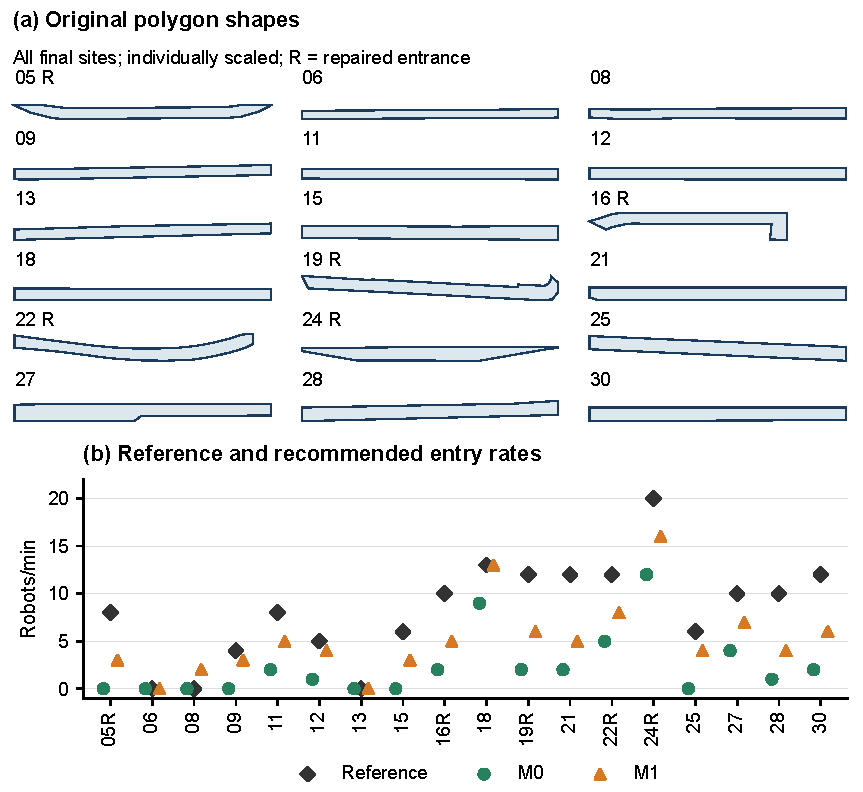
\includegraphics[width=\textwidth]{figures/figure3.pdf}
\caption{Hong Kong geometry transfer. (a) Polygon shapes with independent display scaling and rotation; R marks an entrance-repaired configuration. (b) Reference flows and candidate entry rates using frozen development parameters. Original and repaired configurations are summarized separately in Table~\ref{tab:hk}.}
\label{fig:hk}
\end{figure}

\begin{table}[!htbp]
\centering\caption{Hong Kong admission outcomes, separated by entrance configuration.}
\label{tab:hk}\setlength{\tabcolsep}{3pt}\begin{tabular}{llrrrrrr}
\toprule
Configuration & Method & Positive & Zero & PASS & FAIL & Exceed & $U$ (\%) \\
\midrule
Original & M0 & 7 & 6 & 7 & 0 & 0 & 16.7 \\
Original & M1 & 11 & 2 & 10 & 1 & 1 & 64.6 \\
Original & M2 & 7 & 6 & 7 & 0 & 0 & 8.3 \\
Original & M3 & 7 & 6 & 7 & 0 & 0 & 16.7 \\
Repaired & M0 & 4 & 1 & 4 & 0 & 0 & 20.0 \\
Repaired & M1 & 5 & 0 & 5 & 0 & 0 & 50.0 \\
Repaired & M2 & 2 & 3 & 2 & 0 & 0 & 0.0 \\
Repaired & M3 & 4 & 1 & 4 & 0 & 0 & 20.0 \\
\bottomrule
\end{tabular}

\par\medskip\noindent\raggedright
Original: \HKOriginalN{} configurations, \HKOrigMZeroUtilN{} positive references for $U$. Repaired: \HKRepairedN{} configurations, \HKRepairMZeroUtilN{} positive references for $U$. Exceedance uses every configuration in its stratum.
\end{table}

Among original configurations, M0 gave \HKOrigMZeroPositive{} positives: \HKOrigMZeroPass{} passed and \HKOrigMZeroFail{} failed. M1 gave \HKOrigMOnePositive{} positives, including \HKOrigMOnePass{} passes and \HKOrigMOneFail{} failure. Their utilization was \HKOrigMZeroUtil{}\% and \HKOrigMOneUtil{}\%. Among repaired configurations, all \HKRepairMZeroPositive{} M0 positives and all \HKRepairMOnePositive{} M1 positives passed. M3 matched M0's outcome counts in each stratum. M2 offered fewer positives in the repaired stratum. The pattern again combined the amount of access offered with configuration-specific service outcomes.

\Needspace{4\baselineskip}
\subsection{Sensitivity to Robot and Flow Assumptions}
Robot dimensions and directional composition changed service outcomes at a fixed entry rate (Table~\ref{tab:sensitivity}). Two scenarios were selected by width-order quartiles before the sensitivity runs. At \SensitivityFlow{}~robots/min, the \NarrowWidth{}~m scenario passed \NarrowDefaultPass{}/\SeedN{} seeds with the default robot body and \NarrowLargePass{}/\SeedN{} with the larger body. The \WideWidth{}~m scenario retained \WideLargePass{}/\SeedN{} passes with the larger body. Changing the pedestrian directional split reduced passing seeds to \NarrowDirectionPass{}/\SeedN{} in the narrow scenario and \WideDirectionPass{}/\SeedN{} in the wider scenario.

\begin{table}[!htbp]
\centering\caption{Sensitivity at \SensitivityFlow{}~robots/min for scenarios of width \NarrowWidth{} and \WideWidth{}~m. Each setting has a matching baseline.}
\label{tab:sensitivity}\begin{tabular}{lrrr}
\toprule
Setting & Radius (m) & Narrow: pass/seeds & Wide: pass/seeds \\
\midrule
Default, 50:50 & 0.480 & 30/30 & 30/30 \\
Smaller body, 50:50 & 0.385 & 30/30 & 30/30 \\
Larger body, 50:50 & 0.575 & 0/30 & 30/30 \\
Default body, 75:25 & 0.480 & 28/30 & 29/30 \\
\bottomrule
\end{tabular}

\end{table}

The smaller and larger bodies use interaction radii \SmallRadius{} and \LargeRadius{}~m. Estimators, margins, and service thresholds remain fixed in these checks. Their differing outcomes indicate that the recommendation is tied to robot geometry and pedestrian-flow composition.

Repeated seed blocks also changed service-test results near a service boundary (Table~\ref{tab:replication}). In the preselected DC-063 case, a lower flow could fail when a higher flow passed. The pattern differed between original and independent blocks. This observed acceptance pattern does not establish a genuinely nonmonotonic population pass probability. It supports testing each candidate flow rather than inferring that every lower rate meets the criterion.

\begin{table}[!htbp]
\centering\caption{Boundary case DC-063: passing seeds in original and independent blocks, each with its own baseline mean. Qualification requires \PassN{}/\SeedN{}.}
\label{tab:replication}\begin{tabular}{rrr}
\toprule
Flow (robots/min) & Original: pass/seeds & Independent: pass/seeds \\
\midrule
1 & 30/30 & 28/30 \\
2 & 28/30 & 29/30 \\
3 & 29/30 & 27/30 \\
4 & 26/30 & 25/30 \\
\bottomrule
\end{tabular}

\end{table}

\Needspace{6\baselineskip}
\section{Discussion}
A margin changes the access that a sidewalk offers, not just the error of a fitted curve. It lowers candidate rates within shared admission scenarios and can remove access entirely in others. Some withheld opportunities would pass the service test. Choosing conservativeness involves weighing those lost opportunities against failed pedestrian-service recommendations. Reference error alone does not express that choice. The comparison with M3 suggests that an extra fitted coefficient offers less leverage over aggregate access than the margin in this experiment.

The framework makes these decisions operationally distinct. An out-of-domain case calls for further assessment or a different model. A service-gate zero points to pedestrian conditions or demand that are unsuitable for robot admission. A zero after margin subtraction reflects the allocation rule. A positive candidate specifies a flow for testing under the stated conditions. This structure complements operating permits and fleet limits by making the local service objective part of the entry-rate decision.

Geometry transfer adds an access-design requirement. A polygon can retain its original shape yet require a different entrance anchor for the simulated demand to enter appropriately. Managers applying a segment-level rule would need to specify where robots and pedestrians enter, as well as the width and demand used in the estimate. The Hong Kong results support this configuration-specific approach; they do not measure the coverage of all sidewalks in the city.

Several limits constrain transfer. Robots are represented as circular walking agents, without an independently calibrated yielding or obstacle-avoidance controller. The service criterion measures average walking conditions rather than collision risk or legal right-of-way compliance. Specified regular demand also limits interpretation under arrival bursts or changing pedestrian activity. Completed-trip counts and finite observation windows differ from actual entry measurements, so nominal recommendations must remain distinct from realized throughput.

The finite flow scan and \SeedN{}-seed groups provide evidence at tested conditions. They do not establish a continuous capacity interval or population pass probability. The bootstrap intervals describe site composition rather than all sources of uncertainty. Fixed gates were selected outside the city folds. Hong Kong is a simulation geometry transfer with prior site inspection, and field validation remains necessary. Robot-size and direction-split results identify two conditions that would require reassessment before applying a recommendation to a different operating setting.

\Needspace{6\baselineskip}
\section{Conclusion}
Sidewalk robot admission can be framed as a local service--access decision by linking applicability, pedestrian baseline conditions, and candidate entry rates. On \EvalN{} held-out scenarios, removing the margin increased positive recommendations from \MZeroPositive{} to \MOnePositive{} and observed failed tests from \MZeroFail{} to \MOneFail{}. The additional \MZeroMOnePositive{} opportunities included \WithdrawnPass{} passes and \WithdrawnFail{} failures. An unconstrained width--demand estimator changed aggregate outcomes less than removing the margin. Hong Kong transfer and sensitivity tests linked service outcomes to entrance configuration, robot size, and flow composition. The framework supports service-aware evaluation of candidate entry rates under stated simulation conditions, rather than defining a universal sidewalk capacity.

\bibliography{ascexmpl-new}
\end{document}
